\section{Solución Propuesta}
%%%%%%%%%%%%%%%%%%%%%%%%%%%%%%%%%%%%%%%%%%
% revisado = false
% actualizar alcance considerando memoria de Rodrigo cerda
%%%%%%%%%%%%%%%%%%%%%%%%%%%%%%%%%%%%%%%%%%
A continuación se describen las características y el propósito de la solución propuesto para el problema planteado.

\subsection{Características de la solución}
%Características de la solución: Se describe una solución al problema indicando las principales características o requisitos que debe cumplir. Se describe desde la perspectiva de la ingeniería informática. La solución debe tener correspondencia con el objetivo general del proyecto, por ejemplo, puede ser el desarrollo de un sistema de software, evaluación o comparación de aplicaciones o métodos, desarrollo y/o evaluación de modelo(s) o de una teoría, etc.
Para resolver el problema, se propuso una solución para Android, la cual corresponde a un SDK que incluye las herramientas necesarias para el desarrollo de aplicaciones de terceros relacionadas a VR/AR/MR. El SDK incluye la documentación, APIs y software de configuración. Las APIs permiten activar y desactivar los distintos motores y sensores distribuidos en el guante como también el agregar, quitar y listar dispositivos Bluetooth. El software de configuración permite levantar un servicio Bluetooth en segundo plano, que permita agregar, activar, desactivar y listar dispositivos conectados. También se pueden guardar los perfiles de configuración de los guantes en el dispositivo. Dicha aplicación de configuración soporta  la conexión de múltiples dispositivos,  para lograr utilizar uno o más OpenGlove desde dispositivos móviles.

Cabe destacar que el SDK no implica un costo para los desarrolladores, ni para los usuarios del guante.

Las tecnologías que permiten implementar las características anteriormente mencionadas, son las siguientes:
\begin{itemize}

\item Servicios en segundo plano en Android \footnote{Background service Android: \url{https://developer.android.com/training/run-background-service/create-service.html}}, que permiten mantener un servicio que pueda seguir funcionando mientras otras aplicaciones se estén utilizando en el dispositivo.

\item Websocket \footnote{Websocket: \url{http://websocket.org/aboutwebsocket.html}}, tecnología que proporciona un canal de comunicación bidireccional y full-duplex (información enviada simultáneamente) sobre un único socket TCP. Está diseñada para ser implementada en navegadores y servidores web, pero puede utilizarse por cualquier aplicación cliente/servidor.

\item Bluetooth\footnote{Bluetooth Android: \url{https://developer.android.com/guide/topics/connectivity/bluetooth.html}}, tecnología de red inalámbrica que permite la transmisión de datos entre dispositivos.

\item Xamarin.Forms\footnote{Xamarin.Forms: \url{https://docs.microsoft.com/en-us/xamarin/xamarin-forms/}} tecnología que permite el desarrollo de aplicaciones multiplataforma para iOS y Android. En este proyecto, permite compartir la interfaz de usuario en ambos sistemas operativos de manera nativa y realizar las implementaciones específicas para cada uno.

\end{itemize}

La Figura \ref{fig:propuesta-arquitectura-open-glove} muestra la ubicación del proyecto considerando la arquitectura de OpenGlove. Es importante considerar que las APIs y servicios desarrollados considera Android como alcance.

\begin{figure}[H]
  \begin{center} 
   	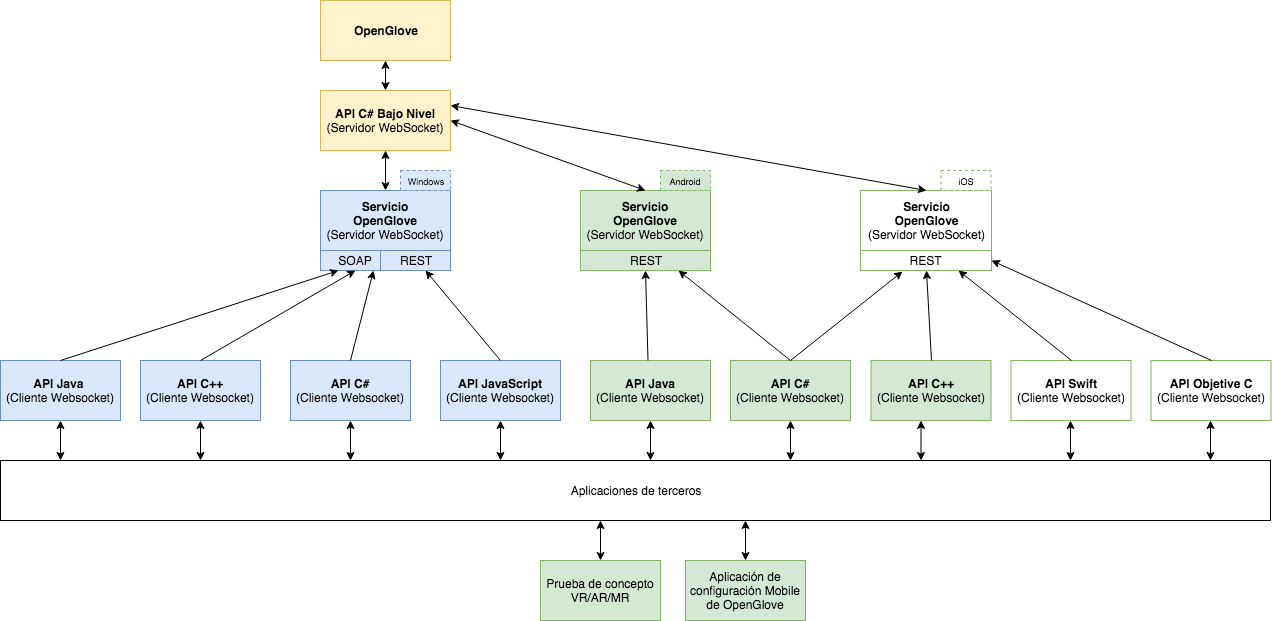
\includegraphics[width=0.9\textwidth]{images/fig-arquitectura/OpenGlove-Architecture-02.png} 
    \caption[Arquitectura Openglove]{Arquitectura OpenGlove \\Fuente: Elaboración propia (2018)}
    \label{fig:propuesta-arquitectura-open-glove}
  \end{center}
\end{figure}

\subsection{Propósitos de la solución}
%Propósito de la solución: Se indica el propósito del producto del proyecto, la razón que justificaría la existencia de una solución. Corresponde a la visión que tiene en mente el cliente respecto de la situación futura, o el beneficio que se espera reciba el destinatario de la solución, indicando en qué medida mejoraría la situación actual del problema.
El propósito del proyecto es poner al alcance de distintas comunidades las herramientas para el desarrollo y uso de dispositivos de respuesta vibrotáctil y seguimiento de las manos en ambientes de realidad virtual, mixta y aumentada, junto con promover el uso de OpenGlove en la comunidad Android, los entusiastas del DIY (Do It Yourself)  o ``házlo tú mismo'' y fabricantes que quieran hacer uso de estas tecnologías para sus proyectos.